% $Id: template.tex 11 2007-04-03 22:25:53Z jpeltier $

\documentclass{vgtc}                          % final (conference style)
%\documentclass[review]{vgtc}                 % review
%\documentclass[widereview]{vgtc}             % wide-spaced review
%\documentclass[preprint]{vgtc}               % preprint
%\documentclass[electronic]{vgtc}             % electronic version

%% Uncomment one of the lines above depending on where your paper is
%% in the conference process. ``review'' and ``widereview'' are for review
%% submission, ``preprint'' is for pre-publication, and the final version
%% doesn't use a specific qualifier. Further, ``electronic'' includes
%% hyperreferences for more convenient online viewing.

%% Please use one of the ``review'' options in combination with the
%% assigned online id (see below) ONLY if your paper uses a double blind
%% review process. Some conferences, like IEEE Vis and InfoVis, have NOT
%% in the past.

%% Figures should be in CMYK or Grey scale format, otherwise, colour 
%% shifting may occur during the printing process.

%% These three lines bring in essential packages: ``mathptmx'' for Type 1 
%% typefaces, ``graphicx'' for inclusion of EPS figures. and ``times''
%% for proper handling of the times font family.

\usepackage{mathptmx}
\usepackage{graphicx}
\usepackage{times}

%% We encourage the use of mathptmx for consistent usage of times font
%% throughout the proceedings. However, if you encounter conflicts
%% with other math-related packages, you may want to disable it.

%% If you are submitting a paper to a conference for review with a double
%% blind reviewing process, please replace the value ``0'' below with your
%% OnlineID. Otherwise, you may safely leave it at ``0''.
\onlineid{0}

%% declare the category of your paper, only shown in review mode
\vgtccategory{Research}

%% allow for this line if you want the electronic option to work properly
\vgtcinsertpkg

%% In preprint mode you may define your own headline.
%\preprinttext{To appear in an IEEE VGTC sponsored conference.}

%% Paper title.

\title{b3.js: A Library for Interactive Virtual Reality Web 3D Graphs}

%% This is how authors are specified in the conference style

%% Author and Affiliation (single author).
%%\author{Roy G. Biv\thanks{e-mail: roy.g.biv@aol.com}}
%%\affiliation{\scriptsize Allied Widgets Research}

%% Author and Affiliation (multiple authors with single affiliations).
%%\author{Roy G. Biv\thanks{e-mail: roy.g.biv@aol.com} %
%%\and Ed Grimley\thanks{e-mail:ed.grimley@aol.com} %
%%\and Martha Stewart\thanks{e-mail:martha.stewart@marthastewart.com}}
%%\affiliation{\scriptsize Martha Stewart Enterprises \\ Microsoft Research}

%% Author and Affiliation (multiple authors with multiple affiliations)
\author{1st Author Name\thanks{e-mail: 1stauthoremail}\\ %
        \scriptsize Affiliation %
\and 2nd Author Name\thanks{e-mail: 2ndauthoremail}\\ %
     \scriptsize Affilation %
\and 3rd Author Name\thanks{e-mail: 3rdauthoremail}\\ %
     \parbox{1.4in}{\scriptsize \centering Affiliation}}

%% A teaser figure can be included as follows, but is not recommended since
%% the space is now taken up by a full width abstract.
%\teaser{
%  \includegraphics[width=1.5in]{}
%  \caption{Lookit! Lookit!}
%}

%% Abstract section.
\abstract{As virtual reality (VR) devices become more ubiquitous and consumer products emerge, libraries are needed to help the design of software that allows VR users manipulate 3D content with comfortable and intuitive motion controls.  We present b3.js, a library for creating interactive VR 3D graphs on a web browser. The 3D graphs, for example,  3D scatter, bar, and surface plots, may be viewed through the Oculus Rift and manipulated with the Leap Motion controller. The Oculus Rift can be used for immersive point of view (POV) perspective within the VR environment. The Leap Motion can be used for controlling the camera zoom level, rotation, and selecting points on the graph for seeing coordinates and point details. We are not aware of any other JavaScript library that provides support for the use of a VR headset and a motion controller to create, view, and interact with 3D graphs in the web browser. Combining the Oculus Rift and Leap Motion enables users to engage in immersive and interactive visualizations of multi-dimensional data, allowing for a novel data exploration experience that is difficult to achieve on a flat screen with the traditional mouse-keyboard paradigm.

} % end of abstract

%% ACM Computing Classification System (CCS). 
%% See <http://www.acm.org/class/1998/> for details.
%% The ``\CCScat'' command takes four arguments.

\CCScatlist{ 
  \CCScat{H.5.1}{Information Interfaces and Presentation}{Multimedia Information Systems}{Artificial, augmented, and virtual realities }
\CCScat{I.3.7}{Computer Graphics}{Three-Dimensional Graphics and Realism}%
{Virtual Reality};
}

%% Copyright space is enabled by default as required by guidelines.
%% It is disabled by the 'review' option or via the following command:
% \nocopyrightspace

%%%%%%%%%%%%%%%%%%%%%%%%%%%%%%%%%%%%%%%%%%%%%%%%%%%%%%%%%%%%%%%%
%%%%%%%%%%%%%%%%%%%%%% START OF THE PAPER %%%%%%%%%%%%%%%%%%%%%%
%%%%%%%%%%%%%%%%%%%%%%%%%%%%%%%%%%%%%%%%%%%%%%%%%%%%%%%%%%%%%%%%%

\begin{document}

%% The ``\maketitle'' command must be the first command after the
%% ``\begin{document}'' command. It prepares and prints the title block.

%% the only exception to this rule is the \firstsection command
\firstsection{Introduction}

\maketitle

%% \section{Introduction} 

Combined with interactive motion sensor hardware like the Leap Motion controller \cite{motion2014leap}, VR devices like the Oculus Rift \cite{oculus2015oculus} can perform together as a new medium and immersive human interface for software \cite{coelho2014pointing}, \cite{khattak2014real}. Research groups within virtual reality and motion sensing hardware specialize in creating 3D environments that act as worlds where users not only virtually perceive but also manipulate environmental objects with seamless, intuitive hand motions \cite{febretti2014omegalib}, \cite{espitia2014development}, \cite{vinkler2014integrating}. Today, when virtual reality and motion controllers are implemented together, the combination is used mostly in video games. Although data visualization in virtual environments have been explored before \cite{helbig2014concept}, VR and motion controllers remain a relatively unexplored combination within development of software such as interactive data visualization. The motivation of b3.js is to expand the usage of VR and motion controllers by providing an interface to visualize and interact with manipulatable datasets in virtual reality.

Data visualization allows us to digest information more effectively. Most graphs provide an immediate overview of data because the main goal is to present information in a visually effective and digestible format. As datasets become larger and more complex, the challenge in data visualization is not only to provide digestible visualization but also new and improved methods of interacting with those visualizations. Although certain information is adequately represented in visualizations on two dimensions, 3D graphs can account for larger and more complicated datasets \cite{ware2008visualizing}. Popular web graphing libraries typically only focus on 2D graphs, which are suitable for simpler line, bar, pie, and clusters that account for two planes or 3D graphs, which need to be visualized on a 2D screen. 2D graphs can effectively visualize data that stays within the x and y coordinate planes. However, too much data under additional variables can overwhelm the limitations of a 2D graph, which can only be seen from one perspective. More appropriately, we require 3D graphs to visualize datasets that consist of more variables than a 2D graph can handle. We live in a three dimensional world where much of our data that we want to decompose and analyze comes from positioning and requires more than two dimensions to represent. In this work, the 3D graphs that we decided to initially focus on were scatter, bar, and surface plots.

\begin{figure}[t]
\begin{center}
   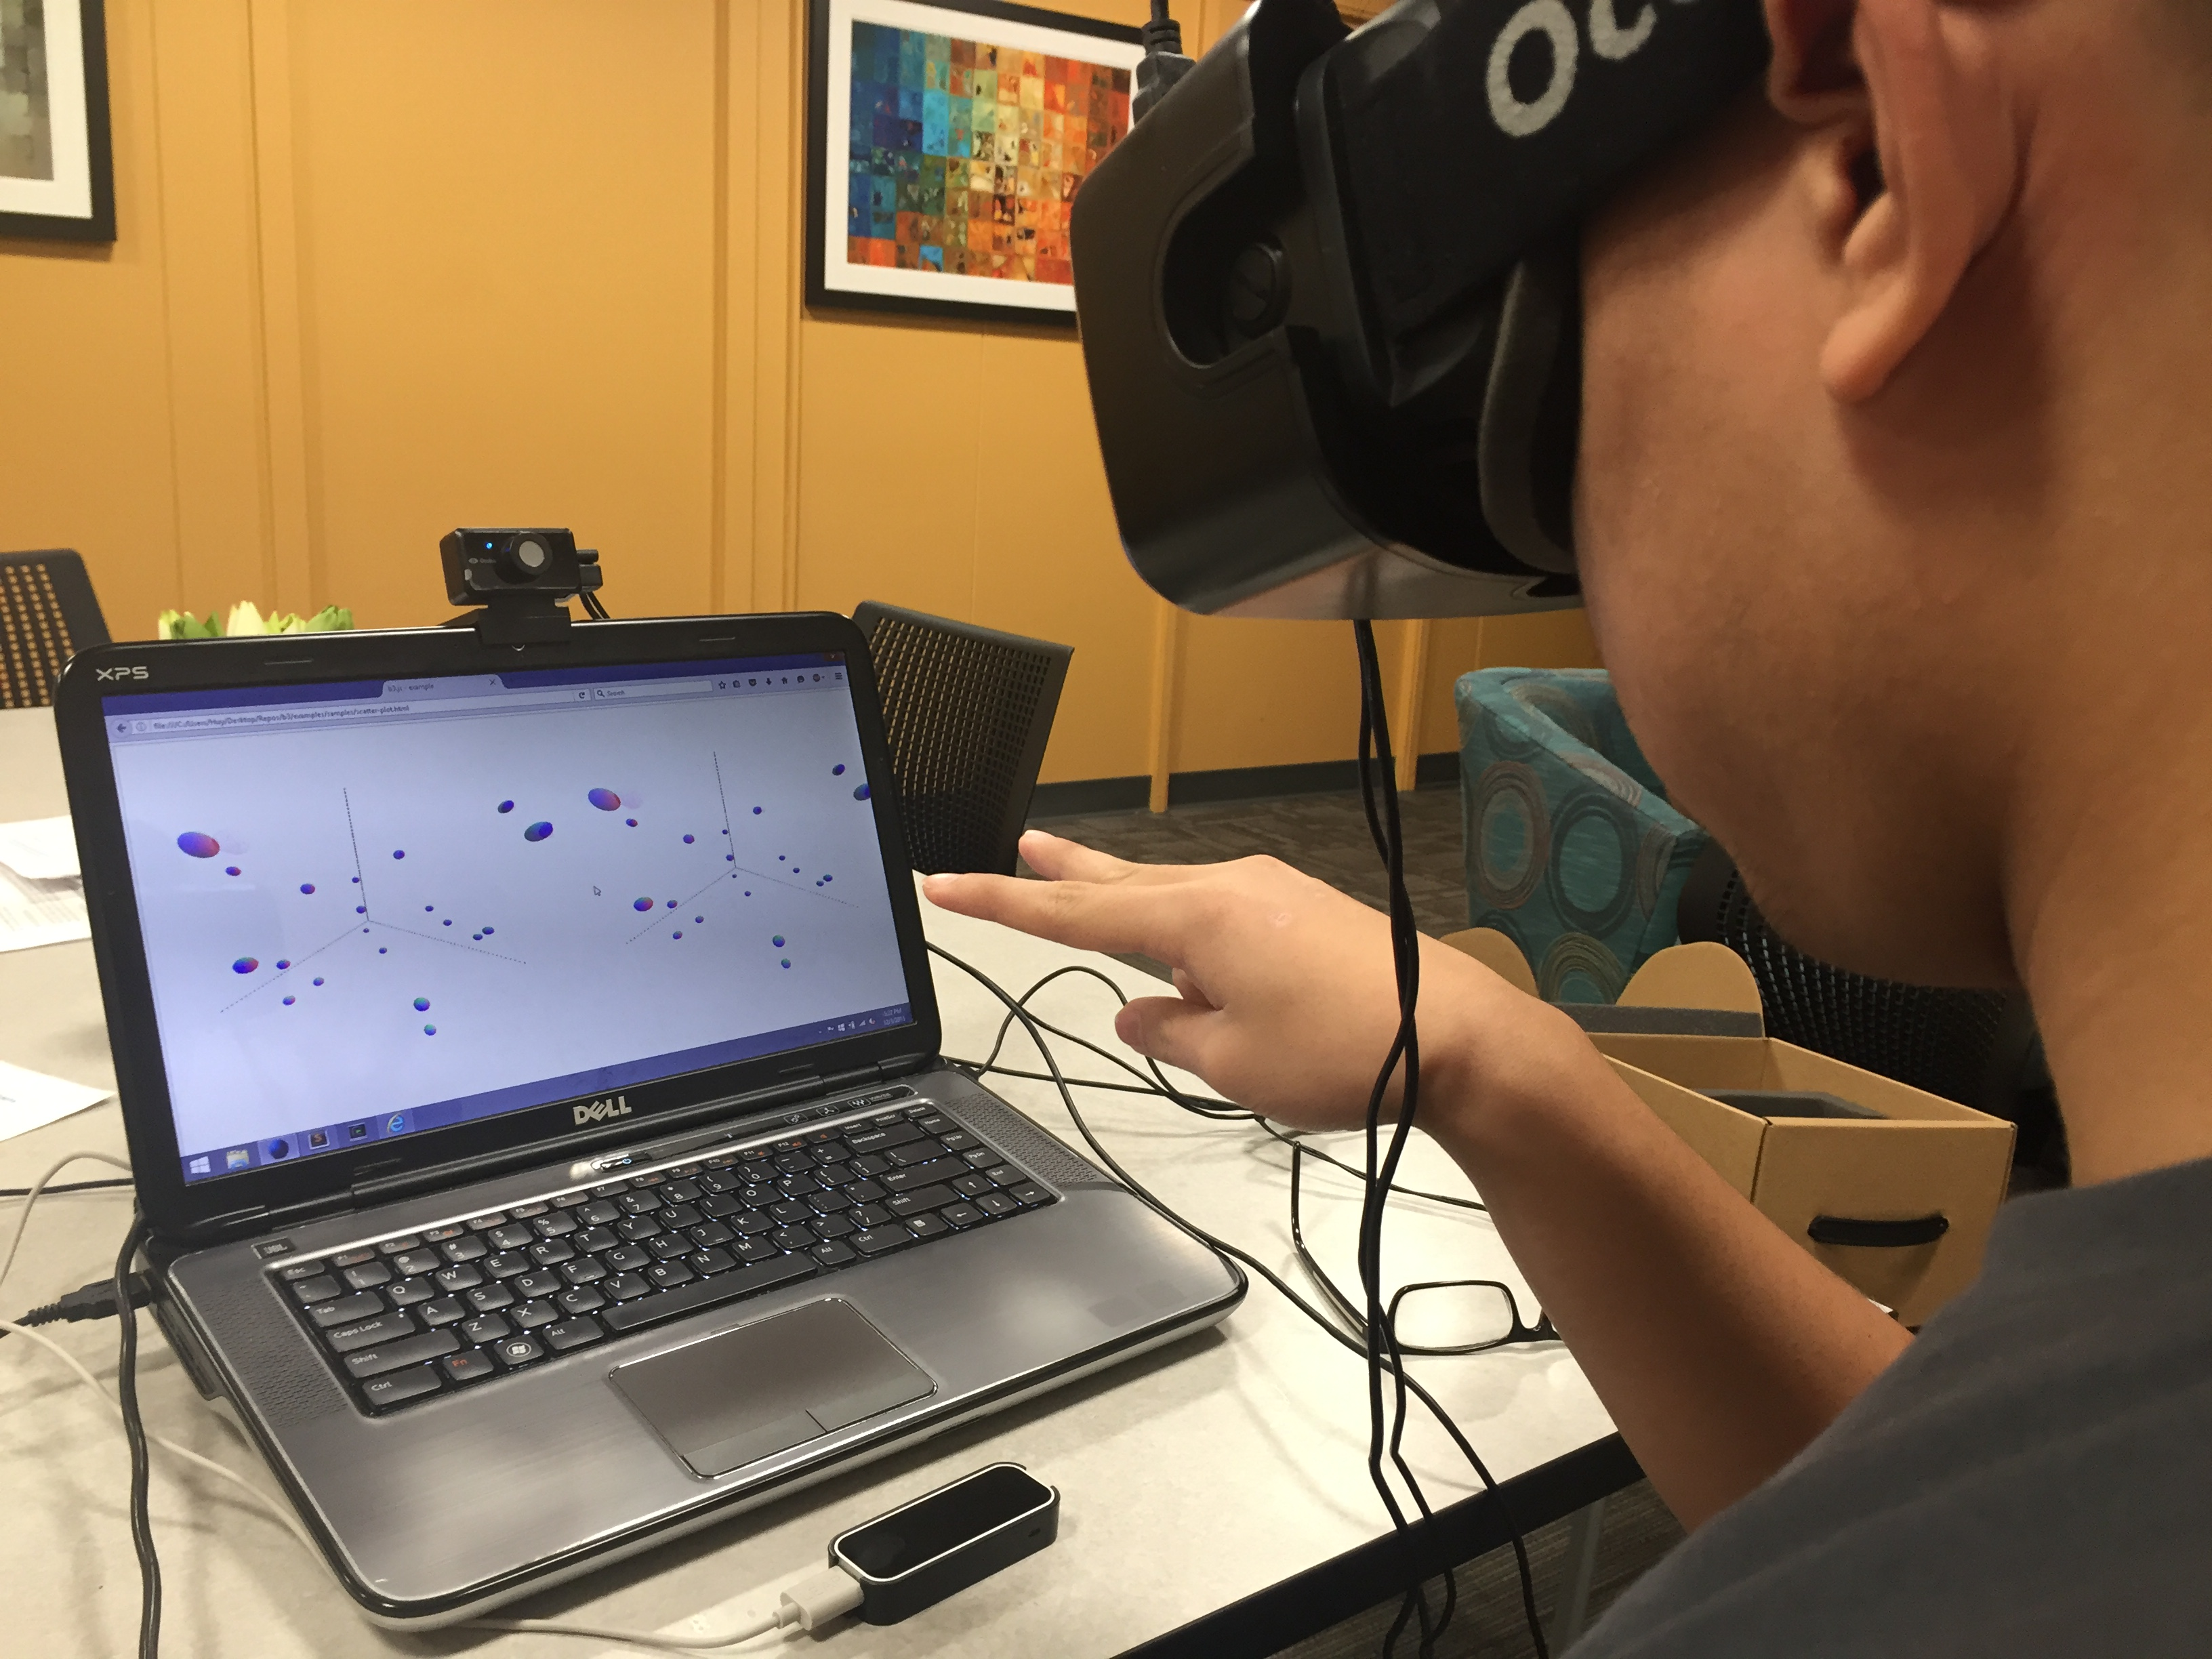
\includegraphics[width=0.7\linewidth]{figure1}
\end{center}
   \caption{A user visualizing and interacting with data on a 3d scatter plot created using b3.js.}
\end{figure}

Interacting with information on 2D planes like reading text from a book is clearly different than interacting on three dimensions like sculpting a statue. What works for interaction on two dimensions to absorb and manipulate information does not transition efficiently when three dimensions exist. We base our motivation for b3.js on our opinions of effective VR in visualization: (1) 3D graphs provide better understanding when the user can control the point of view, (2) 3D graphs are not digested in the same manner as 2D graphs.

We can understand more about the data visualization if we have controls over the perspective with which we are observing. Especially with 3D graphs that rely on the positioning of multiple points, a slight variation of perspective can be deceptive to our appropriate understanding of the data. Although many 3D graphs are rendered as images on the web browser, 3D graphs tend to have perspective controls in the form of mouse manipulation. The novelty of b3.js lies in the inherently immersive experience of visualizing data in a virtual environment. Using b3.js, users can have natural control of a 3D object, such as a graph element, where interaction can be seamless and intuitive. These natural interactions are enabled by the motion controller which tracks the movements of the user’s hands in 3D space. Thus, our focus is to bring immersive controls and interaction through the Oculus Rift and Leap Motion controller to provide motion controlled manipulation of 3D graphs. The immersion and intuitive interactions provide a means of understanding complex datasets that already require a 3D graph on top of a new but increasingly familiar medium of virtual reality and motion controls.

\section{Framework}

\begin{figure}[t]
\begin{center}
   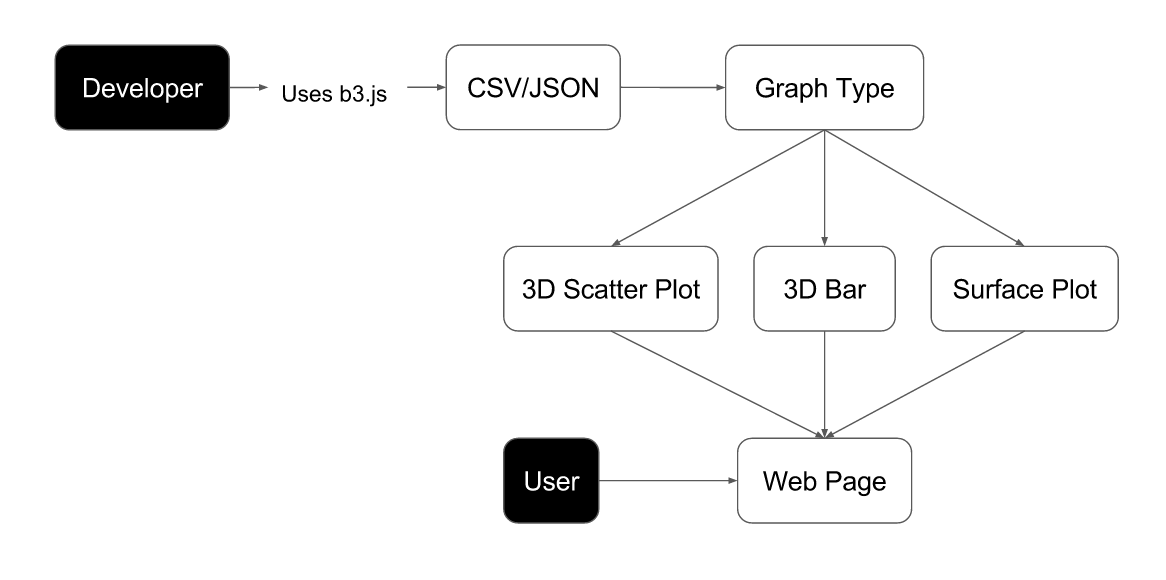
\includegraphics[width=0.75\linewidth]{figure2}
\end{center}
   \caption{Diagram outlining the development process from developer to user.}
\end{figure}

\begin{figure}[t]
\begin{center}
   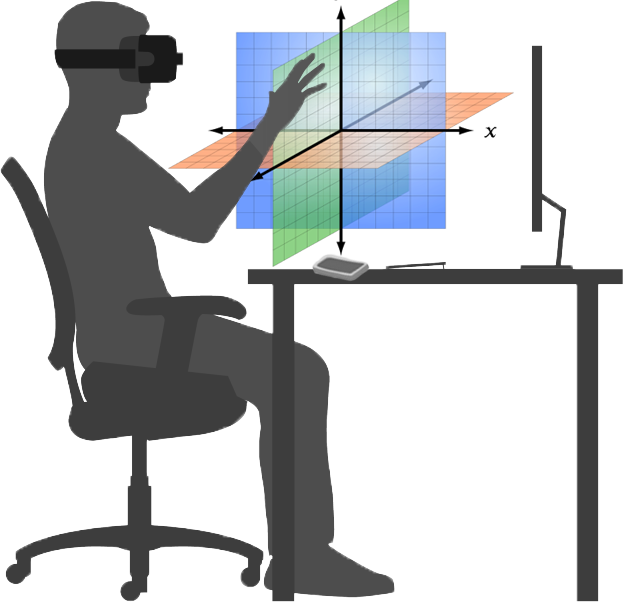
\includegraphics[width=0.75\linewidth]{figure3}
\end{center}
   \caption{How a user would appear while using a b3.js web application.}
\end{figure}

b3.js is meant to be incorporated inside web applications to provide VR and motion control capabilities within generated 3D graphs. Once a developer has downloaded the library, an additional requirement for incorporating the VR is to use a browser capable of detecting VR devices like the Oculus Rift. The two most popular VR enabled browsers are WebVR enabled builds of Google Chromium and Mozilla Firefox. After connecting the JavaScript library to HTML, to create a minimalistic graph, a developer only needs to run initiate(type) and coordinates(name of file). The currently supported graph types are: scatter, bar, and surface with additional support for time series data. The ingested file to extract the coordinates can be of CSV or JSON formats. Other parameters control for establishing names and additional metadata to be incorporating into the graph.

From the user’s perspective, the Oculus Rift and Leap Motion are connected to the computer. The Leap Motion lays in front of the computer. The user wears the Oculus Rift and opens the an application web page rendering a b3.js graph. The web page detects both the Oculus Rift and Leap Motion. From there on, the user can manipulate the camera’s rotation, zoom, and panning with the Leap Motion controller and see the graph in virtual reality immersion.

\section{Functionality}

\begin{figure}[t]
\begin{center}
   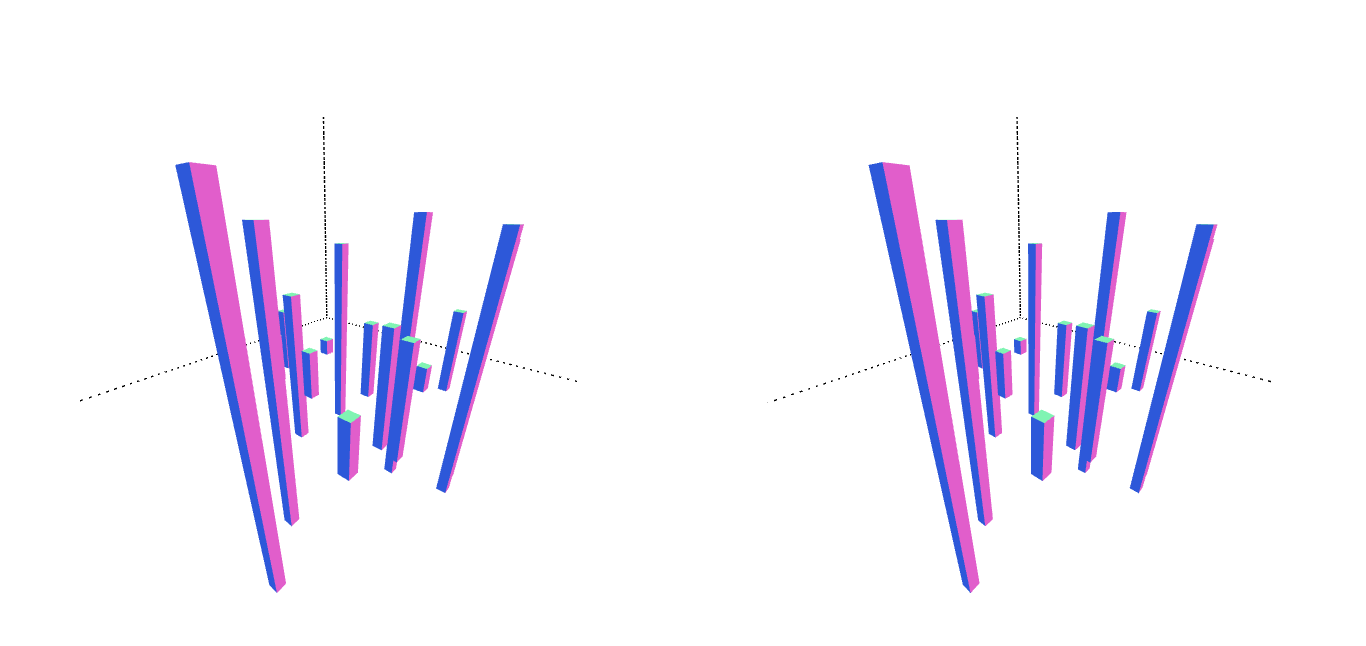
\includegraphics[width=0.75\linewidth]{figure4}
\end{center}
   \caption{An example of a bar graph generated by b3.js}
\end{figure}

\begin{figure}[t]
\begin{center}
   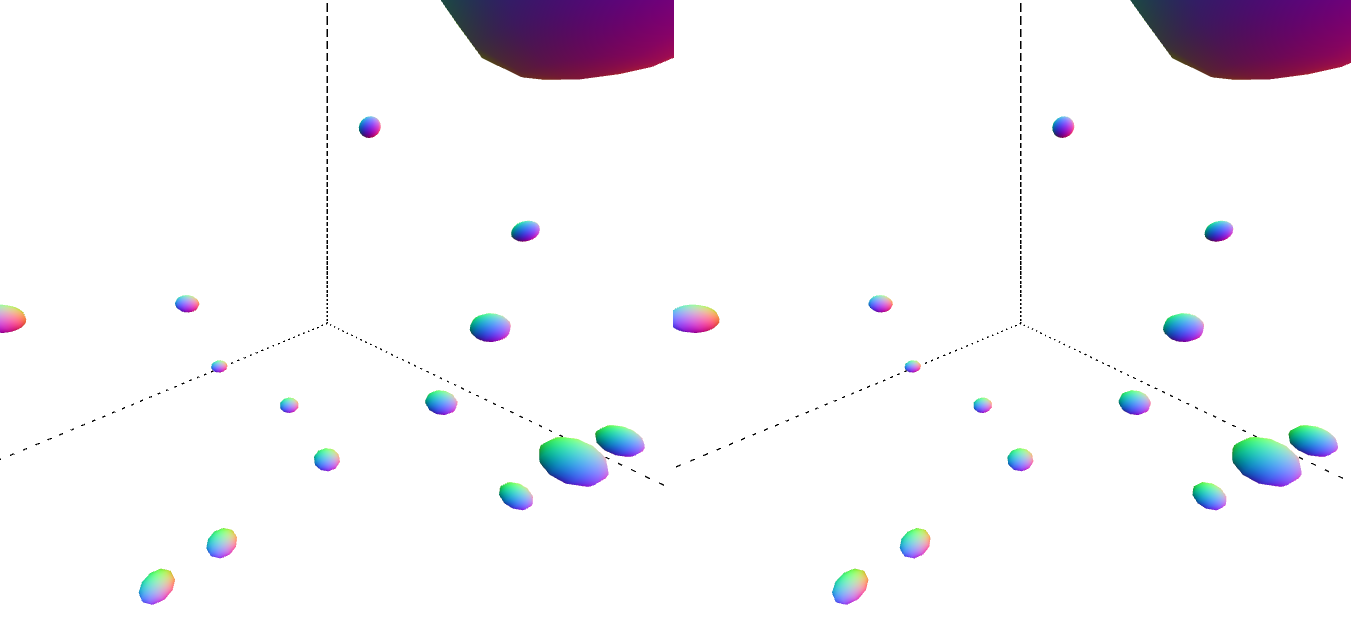
\includegraphics[width=0.75\linewidth]{figure5}
\end{center}
   \caption{An example of a scatter plot generated by b3.js}
\end{figure}

\begin{figure}[t]
\begin{center}
   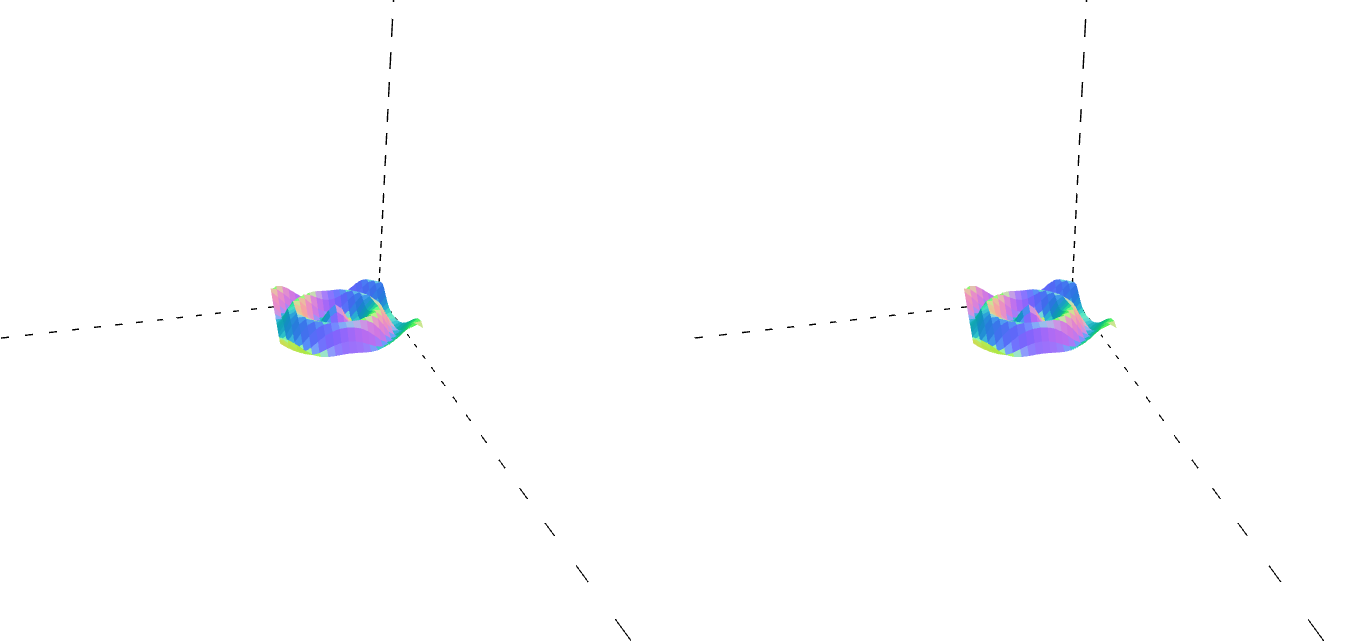
\includegraphics[width=0.75\linewidth]{figure6}
\end{center}
   \caption{An example of a surface plot generated by b3.js}
\end{figure}

Although we saw the opportunity for the creation of a standalone program for generating and observing 3D graphs with VR and motion, we focused b3.js to be a web library to allow anyone with a browser to use it. To create three dimensional objects within the web browser, we used a library known as Three.js ~\cite{cabello2010three} built on top of WebGL. WebGL is a JavaScript API that provides interactive 2D and 3D graphics renderable inside the web browser without the need of plugins. Using Three.js, we created generating functions for ingesting CSV and JSON datasets that could be rendered into 3D graphs.

After the 3D graphs could be generated with the use of functions in the b3.js library, we integrated Oculus Rift and Leap Motion controller support. To incorporate the Oculus Rift, we used two libraries called VREffect.js and VRControls.js, one to replicate the screen into two identical parts required to create the 3D effect and the other to translate head coordinates and movement into camera positioning. For the Leap Motion controller, we used leap.js, a Javascript library for the Leap Motion controller that detects hand and finger positioning. We created controls based on the number of fingers held outward above the Leap Motion. Using a series of listener functions, we divided functionality into three main components: one finger for selection, two fingers for rotation,  two hands for panning, and five fingers for zooming in and out. As well as motion controls, we provided the same camera controls with the mouse.

\section{Implementation}
The main two portions of the b3.js library come from the implementation of virtual reality perspective and motion controls. To start implementing WebVR into the project, there existed a number of WebVR demos available on Github. With VR, the web page must move in response to one’s head movement towards or away from the computer, side to side, or rotate completely. WebVR provides the necessary API to detect and start using virtual reality devices in the web browser. First, we start with detection of the VR device connected to the computer. To detect an array of VR devices connected to the computer, we made use of a WebVR call, Navigator.getVRDevices. Navigator.getVRDevices may return PositionSensorVRDevice, a position sensor camera, or HMDVRDevice, a VR head mounted display. We take advantage of this WebVR call and parse the array for an instance of PositionSensorVRDevice. Since PositionSensorVRDevice inherits the device name, we filter for device names, “oculus” or “cardboard.” 

Once a supported device has been detected, we check the current state of the position sensor by using PositionSensorVRDevice.getState. The state contains the current orientation of the VR device. When the page loads,
 we use PositionSensorVRDevice.resetSensor to calibrate the position and orientation of the VR device and reset to zero. The Rift SDK returns position in meters.

We use HMDVRDevice to sync the left and right eye screens to the proper perspectives inside the VR environment. HMDVRDevice.getEyeParameters returns the current parameters for the “left” or “right” eye as a VREyeParameters object. Once we initialize the VREyeParameters left and right objects, we create additional variables for VREyeParameters.eyeTranslation, which represents the offset from the center of the user’s head to the eye and VREyeParameters.recommendedFieldOfView, which represents the recommended field of view for the current eye. 

We create a full screen renderer, which is the drawing canvas, with Three.js that maps to the entire width and height of the webpage. Then, we add two perspective cameras on the drawing canvas to portray two replicated screens side by side. To display anything in Three.js, we needed to create a scene. The renderer renders the left and right screens for the left and right eyes to the scene. 

With the recommendedFieldOfView object from the left and right eyes, we have the upper, downward, left, and right degrees of each eye. In an update function, we translate this field of vision degrees to radians. To project field of vision to the scene, we take the tangent of each position’s radians, and we scale the positions for normalized device coordinates into an identity matrix. We take the transposed identity matrix to map into the PerspectiveCamera objects for the left and right eyes. The transposed matrices are created because we take the main camera of the VR environment essentially to add the left and right cameras with room for additional cameras for motion controls. We, then, take the left and right eye’s eyeTranslation coordinates to constantly listen and render the eye cameras into the scene. 

The Leap Motion is controlled through its Javascript SDK. When the Leap Motion controller is connected to the computer, we use the Leap.loop function to set up a WebSocket connection for regular update intervals. Leap data taken as frames are passed to a callback function. The frame object contains attributes such as fingers, gestures, and hands. The frame contains separate arrays of pointable, gesture, and hand objects. We separate motion into three main categories: rotation, zoom, and pan. We set the default user as a right handed user. From there, we track for the frame detection of two or three fingers for rotation. Two hands are used for panning. Five fingers are used for zooming. 

To create the controls, we extract the frame to check if the instance of the frame has the correct Pointable and Hand objects. For each of the controls, we take a look at the Hand.palmPosition to grab a unit direction vector that represents the center position of the palm from the Leap. The palm position allows us to identify a left or right hand. We extract the Hand.stablizedPalmPosition as well as the corresponding number of finger Pointable objects. The finger Pointable objects contain Pointable.stablizedTipPosition, which is the tip position from the Leap origin. Processed through conditionals to check for the correct number of fingers and hands for rotation, zooming, and panning, the positions are returned to Three.js cameras that apply the corresponding transformation into the web page.

There are three cameras for rotating, zooming, and panning that ingest the positions of the Hand and Pointable objects. Inside the camera functions, we process the vectors from the positions of hand and fingers. In this processing, we use Three.mapLinear that takes two ranges of numbers, a1 - a2 and b1 - b2, and finds the equivalent positions in range a in b. For rotation, we track the translation into radians. For zooming and panning, we track the translation into the screen’s height and width. For rotating the camera, we create an identity matrix with translations of the finger positions to rotate around three axes. Then, we apply rotation on the camera according to this identity matrix. For zooming and panning the camera, we use the translations of palm and finger positions to create a vector that moves the camera accordingly. For the cursor pointer, we translated a single finger’s tip position into corresponding height and width on the page. The update function constantly listens to the frames and applies the changes to the camera into the rendered scene. By default, we add the addition of mouse controls for rotating, zooming, and panning the graph, which is implemented through a third party library called OrbitControls. 

\section{Generation}

For the generation of 3D bar, scatter, and surface plots, we use functions to change coordinates as graph objects. After ingesting JSON and CSV data, we use conditionals to decide what type of graph the developer wants to create. The camera initializes at the origin where we map the coordinate system with Three.lineGeometry. For bar graphs, we create Three.CubeGeometry objects to create 3D bars for every graph object. For scatter plots, we create Three.SphereGeometry objects to create 3D graph points. For surface plots, we create a series of subVectors and crossVectors to create the 3D surface plot according to data ingested. Every object within the dataset is pushed into an array where we render the array of objects into the scene. Every object also contains a Three.Sprite, which is a plane in a 3D scene that always faces the camera. We put a 3D text box on the sprite that contains the coordinates of the object that is highlighted by either the user’s mouse or finger pointing at the object. 

Each of these graph types also support a time series option. The time series option assumes that the CSV or JSON data is separated into independent subsets. These independent subsets are individually rendered as scenes into the graph one by one. To move to the next subset of data, the user can either press the right arrow key to proceed or the left arrow key to see the previous subset of data. The arrow key controls are implemented with a listener that tracks the keyCode of the button pressed on the keyboard. The user may also perform a swipe gesture left or right with a hand above the Leap Motion to move from subset to subset of data.

\section{Example Application: Visualizing the Collective Flight of Bats}

\begin{figure}[t]
\begin{center}
   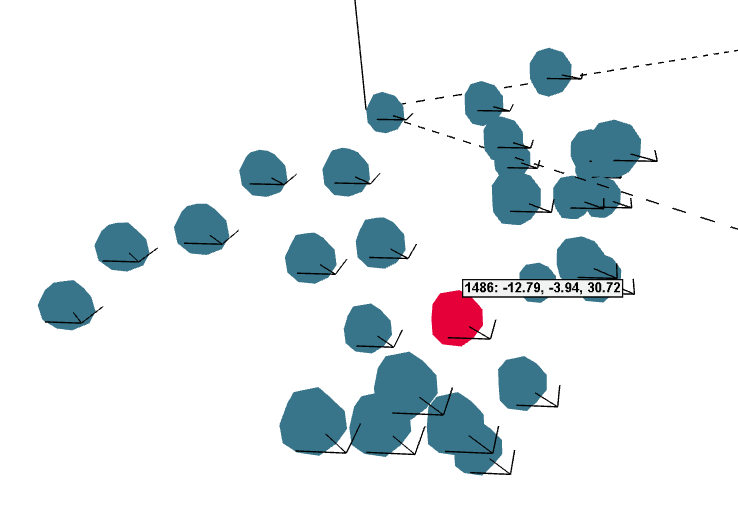
\includegraphics[width=0.75\linewidth]{figure7}
\end{center}
   \caption{A single frame of a time-series scatter-plot visualization of the collective flight of a colony of bats. The red sphere denotes a gesturally selected bat, which triggers a display of information such as 3D coordinates and heading.}
\end{figure}

One of the goals for b3.js is to use the library for real data. An example application that we have developed uses 3D positions of a flock of thousands of bats emerging from a cave over a course of six and a half hours. The main point of research for this bat data was to understand the collective behavior of flying bats. Visualizing the bats in 3D along with immersive VR and motion controls allows us to understand clearly across time how the bats are positioned with respect to their neighbors. We used b3.js to create a 3D time series scatter plot that ingested the trajectories of the bat data in JSON format. With b3.js, we had seamless motion control over perspective to understand the local interactions of bats with their neighbors. Leap Motion one finger selection allowed us to keep track of a particular bat across time. The Oculus Rift and VR component allowed us to detect slight variations of neighboring bats as we could peer over with our heads at particular small groups. Integration of the bat data into b3.js provided a level of control and immersion not possible with existing graph libraries.

\section{Future Work}

In this paper, we described our first version of b3.js, a library for creating interactive VR 3D graphs on the web browser that can be viewed through the Oculus Rift and manipulated with the Leap Motion controller.
A primary future goal for the project is to create a more expansive library with many graph options. In its current version, b3.js can create basic 3D scatter, bar, and surface plots with options for time series and identifying metadata. Although b3.js is easy to use as the functions support reading of files in CSV or JSON format into the graphs that we have provided, we hope to expand the ability for developers to incorporate very specific needs into the graph generation functions such as changing colors, having full control over the coordinate axes, and applying custom inputted points outside of file data. Currently, the developer can apply these additions by adding to the source or custom JavaScript files, but we want to create a more expansive suite of functions that can cater to both specific and general developer needs.

%\begin{figure}[htb]
%  \centering
%  \includegraphics[width=1.5in]{}
%  \caption{Sample illustration.}
%\end{figure}


%% if specified like this the section will be ommitted in review mode
%\acknowledgements{
%The authors wish to thank A, B, C. This work was supported in part by
%a grant from XYZ.}

\bibliographystyle{abbrv}
%%use following if all content of bibtex file should be shown
%\nocite{*}
\bibliography{template}
\end{document}
